\documentclass{article}
\usepackage{graphicx}
\usepackage[utf8]{inputenc}
\usepackage{amsmath, amssymb, latexsym}

\usepackage{pgfplots}
\usepackage{algorithm}
\usepackage[noend]{algpseudocode}
\usepackage{tikz}
\usepackage{nicefrac}
\usepackage{placeins}
\pgfplotsset{every axis legend/.append style={
      at={(0,0)},
      anchor=north east}}
\usetikzlibrary{shapes,positioning,intersections,quotes}
\usetikzlibrary{arrows.meta,
  bending,
  intersections,
  quotes,
  shapes.geometric}

\definecolor{darkgreen}{rgb}{0.0, 0.6, 0.0}
\definecolor{darkred}{rgb}{0.7, 0.0, 0.0}
\makeatletter
\def\BState{\State\hskip-\ALG@thistlm}
\makeatother
\title{Week 16}
\begin{document}
\pagenumbering{gobble}
\maketitle
\newpage
\pagenumbering{arabic}

\section*{Recommender systems}

\begin{itemize}
  \item Many technological businesses consider recommender systems to be critical (amazon, Ebay, iTunes genius).
  \item Based on previous purchases, try to propose new content to you.
  \item It's not so much a method as it is a concept.
\end{itemize}

Example: predict movie ratings.

\begin{itemize}
  \item You work at a firm that sells movies.
  \item You allow viewers to rate movies on a scale of 1 to 5.
  \item You have five films.
  \item You also have four users.
\end{itemize}

~\\
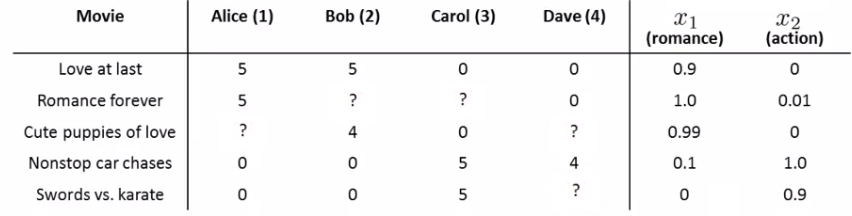
\includegraphics[width=\textwidth]{resources/movie_recommendation}

\begin{itemize}
  \item $n_u$ - number of users.
  \item $n_m$ - number of movies.
  \item $r(i,j)$ -  1 if user j has rated movie i.
  \item  $y^{(i,j)}$ - rating given by user j to move i.
  \item If we have features like this, a feature vector may recommend each film.
  \item For each film, add an additional feature that is x0 = 1.
  \item So we have a $[3 \times 1]$ vector for each film, which for film number three ("Cute Puppies of Love") would be:
\end{itemize}

\begin{align*}
  x^{(3)} & = \begin{bmatrix}
    1    \\
    0.99 \\
    0
  \end{bmatrix}
\end{align*}

So, let's take a look at user 1 (Alice) and see what she thinks of the modern classic Cute Puppies of Love (CPOL). She is associated with the following parameter vector:

\begin{align*}
  \theta^{(1)} & = \begin{bmatrix}
    0 \\
    5 \\
    0
  \end{bmatrix}
\end{align*}

~\\
Our prediction:

$$(\theta^1)^Tx^3 = (0\cdot1)+(5\cdot0.99)+(0\cdot0)=4.95$$

\section*{How do we learn $(\theta^j)$?}

This is analogous to linear regression with least-squares error:

$$min_{\theta^j} = \frac{1}{2m^{(j)}}\sum_{i:r(i,j)=1}((\theta^{(j)})^T(x^{(i)})-y^{(i,j)})^2+\frac{\lambda}{2m^{(j)}}\sum_{k=1}^{n}(\theta_k^{(j)})^2$$

We have the gradient descent algorithm to find the minimum:

$$\theta_k^{(j)} := \theta_k^{(j)}-\alpha \sum_{i:r(i,j)=1}((\theta^{(j)})^T(x^{(i)})-y^{(i,j)})x_k^{(i)}\ (for\ k=0)$$
$$\theta_k^{(j)} := \theta_k^{(j)}-\alpha( \sum_{i:r(i,j)=1}((\theta^{(j)})^T(x^{(i)})-y^{(i,j)})x_k^{(i)} + \lambda \theta_k^{(j)})\ (for\ k\neq0)$$

\section*{Collaborative filtering}
The collaborative filtering algorithm has a very intriguing property: it can learn what characteristics it needs to learn for itself.

~\\
If we are given user preferences ($\theta^{(1)}, ...,\theta^{(n_u)}$) we may use them to find out the film's features ($x^{(1)}, ...,x^{(n_m)}$) and vice versa:

$$min_{x^{(1)}, ...,x^{(n_m)}} \frac{1}{2} \sum_{i=1}^{n_m} \sum_{i:r(i,j)=1}((\theta^{(j)})^T(x^{(i)})-y^{(i,j)})^2+\frac{\lambda}{2}\sum_{i=1}^{n_m}\sum_{k=1}^{n}(x_k^{(i)})^2$$

One thing you could do is:
\begin{itemize}
  \item Randomly initialize parameter.
  \item Go back and forth in time.
\end{itemize}

\section*{Vectorization: Low rank matrix factorization}

How can we enhance the collaborative filtering algorithm now that we've looked at it?

~\\
So, in our previous example, take all ratings from all users and organize them into a matrix Y.

~\\
5 movies and 4 users, give us a $[5 \times 4]$ matrix:

\begin{equation*}
  Y =
  \begin{pmatrix}
    5 & 5 & 0 & 0 \\
    5 & ? & ? & 0 \\
    ? & 4 & 0 & ? \\
    0 & 0 & 5 & 4 \\
    0 & 0 & 5 & 0
  \end{pmatrix}
\end{equation*}

~\\
Given [Y] there's another way of writing out all the predicted ratings:

\begin{equation*}
  X \cdot \Theta^T =
  \begin{pmatrix}
    (\theta^{(1)})^T(x^{(1)})   & (\theta^{(2)})^T(x^{(1)})   & ...    & (\theta^{(n_u)})^T(x^{(1)})   \\
    (\theta^{(1)})^T(x^{(2)})   & (\theta^{(2)})^T(x^{(2)})   & ...    & (\theta^{(n_u)})^T(x^{(2)})   \\
    \vdots                      & \vdots                      & \vdots & \vdots                        \\
    (\theta^{(1)})^T(x^{(n_m)}) & (\theta^{(2)})^T(x^{(n_m)}) & ...    & (\theta^{(n_u)})^T(x^{(n_m)})
  \end{pmatrix}
\end{equation*}

~\\
Where matrix X is constructed by taking all the features for each movie and stacking them in rows:

\begin{align*}
  X & = \begin{bmatrix}
    -(x^{(1)})^T-   \\
    -(x^{(2)})^T-   \\
    \vdots          \\
    -(x^{(n_m)})^T-
  \end{bmatrix}
\end{align*}

And matrix $\Theta$ is constructed by taking all the features for each movie and stacking them in rows:

\begin{align*}
  \Theta & = \begin{bmatrix}
    -(\theta^{(1)})^T-   \\
    -(\theta^{(2)})^T-   \\
    \vdots               \\
    -(\theta^{(n_u)})^T-
  \end{bmatrix}
\end{align*}

\section*{Mean Normalization}

Consider a user who hasn't reviewed any movies.

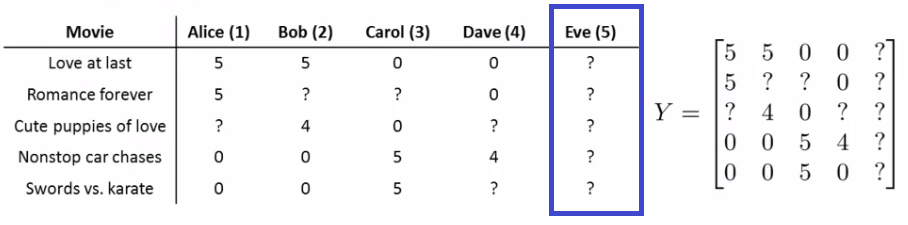
\includegraphics[width=\textwidth]{resources/no_ratings}

\begin{itemize}
  \item There are no films for which r(i,j) = 1.
  \item So this term places no role in determining $\theta^5$.
  \item So we're just minimizing the final regularization term.
\end{itemize}

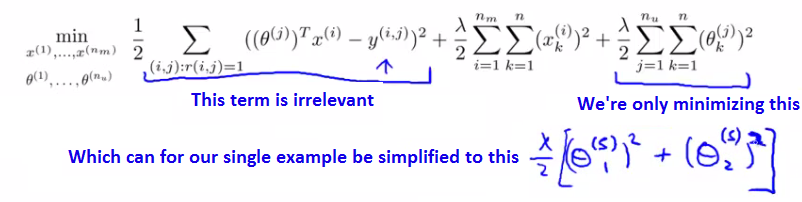
\includegraphics[width=\textwidth]{resources/no_ratings_formula}

\begin{itemize}
  \item As previously, put all of our ratings into matrix Y.
  \item We now compute the average rating for each movie and store it in a $n_m$ - dimensional column vector.

        \begin{align*}
          \mu & = \begin{bmatrix}
            2.5  \\
            2.5  \\
            2    \\
            2.25 \\
            1.25
          \end{bmatrix}
        \end{align*}

  \item If we take a look at all of the movie ratings in [Y], we can subtract the mean rating.

        \begin{equation*}
          Y =
          \begin{pmatrix}
            2.5   & 2.5   & -2.5 & -2.5  & ? \\
            2.5   & ?     & ?    & -2.5  & ? \\
            ?     & 2     & -2   & ?     & ? \\
            -2.25 & -2.25 & 2.75 & 1.75  & ? \\
            -1.25 & -1.25 & 3.75 & -1.25 & ?
          \end{pmatrix}
        \end{equation*}

  \item That is, we normalize each film to have an average rating of 0.

\end{itemize}


\end{document}
